\documentclass[journal,12pt,onecolumn]{IEEEtran}
\usepackage{cite}
\usepackage{graphicx}
\usepackage{amsmath,amssymb,amsfonts,amsthm}
\usepackage{algorithmic}
\usepackage{graphicx}
\usepackage{textcomp}
\usepackage{xcolor}
\usepackage{txfonts}
\usepackage{listings}
\usepackage{enumitem}
\usepackage{mathtools}
\usepackage{gensymb}
\usepackage{comment}
\usepackage[breaklinks=true]{hyperref}
\usepackage{tkz-euclide} 
\usepackage{listings}
\usepackage{gvv}                                        
%\def\inputGnumericTable{}                                 
\usepackage[latin1]{inputenc}
\usetikzlibrary{arrows.meta, positioning}
\usepackage{xparse}
\usepackage{color}                                            
\usepackage{array}                                            
\usepackage{longtable}                                       
\usepackage{calc}                                             
\usepackage{multirow}
\usepackage{multicol}
\usepackage{hhline}                                           
\usepackage{ifthen}                                           
\usepackage{lscape}
\usepackage{tabularx}
\usepackage{array}
\usepackage{float}
\newtheorem{theorem}{Theorem}[section]
\newtheorem{problem}{Problem}
\newtheorem{proposition}{Proposition}[section]
\newtheorem{lemma}{Lemma}[section]
\newtheorem{corollary}[theorem]{Corollary}
\newtheorem{example}{Example}[section]
\newtheorem{definition}[problem]{Definition}
\newcommand{\BEQA}{\begin{eqnarray}}
\newcommand{\EEQA}{\end{eqnarray}}
\usepackage{float}
%\newcommand{\define}{\stackrel{\triangle}{=}}
\theoremstyle{remark}
\usepackage{circuitikz}
\usepackage{tikz}
\usepackage{ragged2e}
\begin{document}

\title{GATE Petroleum Engineering (PE) 2024}
\maketitle
\section*{General Aptitude (GA)}
\begin{enumerate}
    \item The fishermen, \_\_\_\_\_ the flood victims owed their lives, were rewarded by the government.
   \begin{enumerate}
       \item whom 
       \item to which
       \item to whom
       \item  that
   \end{enumerate}
      \hfill{GATE PE 2020}
   
    \item Some students were not involved in the strike. If the above statement is true, which of the following conclusions is/are logically necessary?
    
    \begin{enumerate}
        \item Some who were involved in the strike were students.
        \item No student was involved in the strike.
        \item At least one student was involved in the strike.
        \item Some who were not involved in the strike were students.
    \end{enumerate}
     \begin{enumerate}
         \item a and b
         \item c
         \item d
         \item b and c
     \end{enumerate} 
      \hfill{GATE PE 2020}
    
    \item The radius as well as the height of a circular cone increases by $10\%$. The percentage increase in its volume is \_\_\_\_\_.
    \begin{enumerate}
        \item 17.1
        \item 21.0
        \item 33.1 
        \item  72.8
    \end{enumerate}
      \hfill{GATE PE 2020}
    
    \item Five numbers 10, 7, 5, 4 and 2 are to be arranged in a sequence from left to right following the directions given below:
    
    \begin{enumerate}
        \item No two odd or even numbers are next to each other.
        \item The second number from the left is exactly half of the left-most number.
        \item The middle number is exactly twice the right-most number.
    \end{enumerate}
    
    Which is the second number from the right?
    \begin{enumerate}
    \begin{multicols}{4}
        \item 2
        \item 4
        \item 7
        \item 10
    \end{multicols}
    \end{enumerate}
      \hfill{GATE PE 2020}
    \item Until Iran came along, India had never been \_\_\_\_\_ in kabaddi.
    \begin{enumerate}
    \begin{multicols}{2}
     \item defeated
     \item defeating
     \item defeat
     \item defeatist
    \end{multicols}
\end{enumerate}
      \hfill{GATE PE 2020}

    \item Since the last one year, after a 125 basis point reduction in repo rate by the Reserve Bank of India, banking institutions have been making a demand to reduce interest rates on small saving schemes. Finally, the government announced yesterday a reduction in interest rates on small saving schemes to bring them on par with fixed deposit interest rates.
    
    Which one of the following statements can be inferred from the given passage?
    \begin{enumerate}
    
        \item  Whenever the Reserve Bank of India reduces the repo rate, the interest rates on small saving schemes are also reduced 
        \item  Interest rates on small saving schemes are always maintained on par with fixed deposit interest rates
        \item The government sometimes takes into consideration the demands of banking institutions before reducing the interest rates on small saving schemes
        \item  A reduction in interest rates on small saving schemes follow only after a reduction in repo rate by the Reserve Bank of India
   
    \end{enumerate}
   
      \hfill{GATE PE 2020}
    \item In a country of 1400 million population, $70\%$ own mobile phones. Among the mobile phone owners, only 294 million access the Internet. Among these Internet users, only half buy goods from e-commerce portals. What is the percentage of these buyers in the country?
    \begin{enumerate} \begin{multicols}{2}
\item 10.50
\item 14.70
\item 15.00
\item 50.00
    \end{multicols} \end{enumerate}
   
      \hfill{GATE PE 2020}
      
    \item The nomenclature of Hindustani music has changed over the centuries. Since the medieval period dhrupad styles were identified as baanis. Terms like gayaki and baaj were used to refer to vocal and instrumental styles, respectively. With the institutionalization of music education the term gharana became acceptable. Gharana originally referred to hereditary musicians from a particular lineage, including disciples and grand disciples.
    
    Which one of the following pairings is NOT correct?
    \begin{enumerate} \begin{multicols}{2}
    \item  dhrupad, baani
    \item  gayaki, vocal
    \item  baaj, institution
    \item  gharana, lineage
    \end{multicols} \end{enumerate}
   
      \hfill{GATE PE 2020}
    
    \item Two trains started at 7AM from the same point. The first train travelled north at a speed of $80$ km/h and the second train travelled south at a speed of $100$ km/h. The time at which they were $540$ km apart is \_\_\_\_\_ AM.
    \begin{enumerate} \begin{multicols}{2}
    \item 9
    \item 10
    \item 11
    \item 11.30
    \end{multicols} \end{enumerate}
    
      \hfill{GATE PE 2020}
     
    \item "I read somewhere that in ancient times the prestige of a kingdom depended upon the number of taxes that it was able to levy on its people. It was very much like the prestige of a head-hunter in his own community."
    
    Based on the paragraph above, the prestige of a head-hunter depended upon 
    \begin{enumerate} \begin{multicols}{2}
\item the prestige of the kingdom
\item the prestige of the heads
\item the number of taxes he could levy
\item the number of heads he could gather
    \end{multicols} \end{enumerate}
    
      \hfill{GATE PE 2020}



\section*{GATE 2019 Petroleum Engineering}




\setcounter{enumi}{10} % Start from question 11

\item Match the following:

\begin{table}[h!]
\centering
\begin{align}
\begin{array}{ll}
P.\; \text{Bingham plastic}            & I.\; \tau = \tau_y + \mu_p \dot{\gamma} \\
Q.\; \text{Power law}                  & II.\; \tau = k y^n \\
R.\; \text{Power law with yield stress} & III.\; \tau = \tau_y + k y^n \\
\end{array}
\end{align}
\caption{Matching of rheological models with their constitutive equations}
\label{tab:rheology}
\end{table}


Here: \\
$\tau$: shear stress \\
$\tau_y$: yield value or yield stress \\
$\mu_p$: shear viscosity \\
$n$: power law index \\
$k$: consistency index \\
$\dot{\gamma}$: shear rate \\
 \begin{enumerate} \begin{multicols}{2}
\item P-II, Q-I, R-III
\item  P-I, Q-III, R-II
\item P-III, Q-II, R-I
\item  P-III, Q-I, R-II
 \end{multicols} \end{enumerate}

  \hfill{GATE PE 2020}
 
\item Match the following for drill pipe failure:

\begin{table}[h!]
\centering
\begin{align}
\begin{array}{ll}
P.\; \text{Twist off} & I.\; \text{due to excessive torque} \\
Q.\; \text{Parting}   & II.\; \text{due to excessive tension} \\
R.\; \text{Collapse}  & III.\; \text{due to extensive external pressure} \\
S.\; \text{Fatigue}   & IV.\; \text{due to cyclic loading} \\
\end{array}
\end{align}
\caption{Failure modes and their causes}
\label{tab:failures}
\end{table}


\begin{multicols}{2}
\begin{enumerate}
\item (A) P-III, Q-IV, R-I, S-II
\item (B) P-II, Q-I, R-IV, S-III
\item (C) P-I, Q-II, R-III, S-IV
\item (D) P-IV, Q-III, R-II, S-I
\end{enumerate}
\end{multicols}


  \hfill{GATE PE 2020}
 
\item Which one of the following flow regimes is more favorable for gas lift operation?

\begin{multicols}{2}
\begin{enumerate}
\item (A) Bubbly flow
\item (B) Annular flow
\item (C) Churn flow
\item (D) Stratified flow
\end{enumerate}
\end{multicols}


  \hfill{GATE PE 2020}

\item H$_2$S gas is

\begin{multicols}{2}
\begin{enumerate}
\item (A) acidic.
\item (B) non-corrosive.
\item (C) lighter than air.
\item (D) non-flammable.
\end{enumerate}
\end{multicols}


  \hfill{GATE PE 2020}

\item Which one of the following offshore platforms DOES NOT use buoyant columns or pontoons?

\begin{multicols}{2}
\begin{enumerate}
\item (A) Tension leg platforms
\item (B) Jack up platforms
\item (C) Spar platforms
\item (D) Semi-submersible platforms
\end{enumerate}
\end{multicols}


  \hfill{GATE PE 2020}
 
\item In which one of the following offshore platforms, the condition of the sea floor is a vital consideration?

\begin{multicols}{2}
\begin{enumerate}
\item (A) Drill ship platforms
\item (B) Tension leg platforms
\item (C) Concrete gravity platforms
\item (D) Floating, production, storage and offloading (FPSO) platforms
\end{enumerate}
\end{multicols}

 
  \hfill{GATE PE 2020}

\item The 'Klinkenberg effect' is related to

\begin{enumerate}
\item (A) viscous fingering during water flooding in oil reservoirs.
\item (B) hysteresis effect in relative permeability during drainage and imbibition process.
\item (C) oil viscosity dependence on temperature.
\item (D) slippage of gas ph
\end{enumerate}

  \hfill{GATE PE 2020}
 
\item Favorable conditions for formation of gas hydrates are

\begin{multicols}{2}
\begin{enumerate}
\item (A) high temperature and high pressure.
\item (B) high temperature and low pressure.
\item (C) low temperature and high pressure.
\item (D) low temperature and low pressure.
\end{enumerate}
\end{multicols}

  \hfill{GATE PE 2020}
   
\item Match the following quantities with their dimensions:

\begin{table}[h!]
\centering
\[
\begin{array}{ll}
P.\; \text{Viscosity}        & I.\; M^{1}L^{-1}T^{-1} \\
Q.\; \text{Permeability}     & II.\; M^{0}L^{2}T^{0} \\
R.\; \text{Compressibility}  & III.\; M^{-1}L^{1}T^{2} \\
S.\; \text{Pressure}         & IV.\; M^{1}L^{-1}T^{-2} \\
\end{array}
\]
\caption{Physical quantities with their dimensional formulas}
\label{tab:dimensions}
\end{table}

   
\begin{multicols}{2}
\begin{enumerate}
\item (A) P-III, Q-II, R-IV, S-I
\item (B) P-II, Q-I, R-IV, S-III
\item (C) P-III, Q-I, R-IV, S-II
\item (D) P-I, Q-II, R-III, S-IV
\end{enumerate}
\end{multicols}

  \hfill{GATE PE 2020}
   
\item The plot of dissolved gas oil ratio (R$_s$), defined as the "ratio of STP volume of gas dissolved in the oil at pressure P, to the volume of the oil at STP" is given below.
\begin{figure}[h]
    \centering
    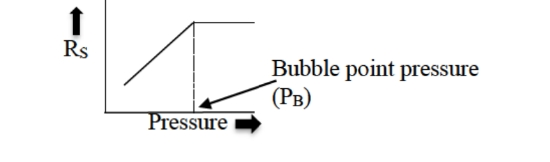
\includegraphics[width=0.5\linewidth]{figs/1.jpeg}
    \caption{}
    \label{fig:placeholder}
\end{figure}

\begin{center}
[Insert Figure: Plot of R$_s$ vs Pressure with Bubble point pressure marked]
\end{center}

For the same oil, the plot of produced gas oil ratio (R$_p$) defined as the "ratio of STP volume of the gas liberated from the oil at pressure P, to the volume of the oil at STP" is
\begin{figure}[h]
    \centering
    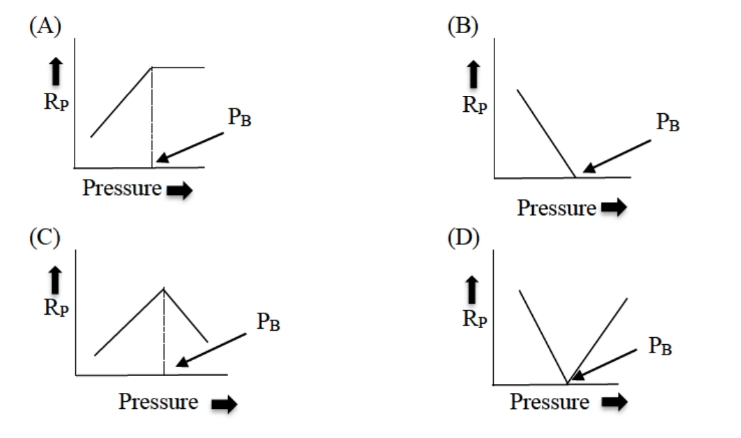
\includegraphics[width=0.5\linewidth]{figs/2.jpeg}
    \caption{}
    \label{fig:placeholder}
\end{figure}

\begin{multicols}{2}
\begin{enumerate}
\item (A) [Figure A]
\item (B) [Figure B]
\item (C) [Figure C]
\item (D) [Figure D]
\end{enumerate}
\end{multicols}


  \hfill{GATE PE 2020}
  

\section*{GATE 2019 Petroleum Engineering}




\item Which one of the following denotes a regular four-spot flood pattern?

\noindent A represents injection well \\
\noindent o represents production well \\
\begin{figure}[h]
    \centering
    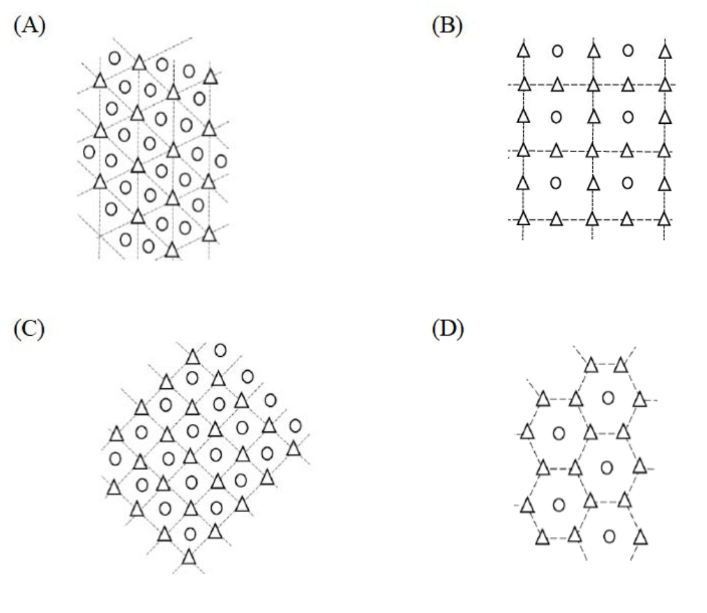
\includegraphics[width=0.5\linewidth]{figs/3.jpeg}
    \caption{}
    \label{fig:placeholder}
\end{figure}


  \hfill{GATE PE 2020}
   
\item The value of $\lim\limits_{x \to 0} \frac{(x+1)\sin x}{x^2 + 2x}$ is  (round off to 2 decimal places).

   Numerical answer

  \hfill{GATE PE 2020}

\item Let $A = \myvec{1 & 2 \\ 2 & 1 }$, $X = \myvec{ 1 & a \\ b & 0 }$ and $Y = \myvec{ 3 & 1 \\ 3 & 2 }$. If $AX = Y$, then $a + b$ equals .

   Numerical answer

  \hfill{GATE PE 2020}
   
\item Let $\vec{u} = \hat{i} + \hat{j} + a\hat{k}$ and $\vec{v} = a^2\hat{i} + 4\hat{j} - 4\hat{k}$, where $\hat{i}, \hat{j}$ and $\hat{k}$ are cartesian unit vectors. If $\vec{u}$ is perpendicular to $\vec{v}$, then $a$ equals \\\\\_.

   Numerical answer

  \hfill{GATE PE 2020}
   
\item If the neutron log porosity ($\phi_N$) is 0.09 and density log porosity ($\phi_D$) is 0.24 in the cross-over region, then the average porosity of the gas bearing region is \\\\\_ (round off to 2 decimal places).

   Numerical answer

  \hfill{GATE PE 2020}

   



\item The general solution of the differential equation $\frac{d^2 y}{dx^2} - 2 \frac{dy}{dx} + y = 0$ is (here $C_1$ and $C_2$ are arbitrary constants)

\begin{multicols}{2}
\begin{enumerate}
\item (A) $y = C_1 e^x + C_2 e^{-x}$
\item (B) $y = C_1 xe^x + C_2 xe^{2x}$
\item (C) $y = C_1 e^x + C_2 xe^{-x}$
\item (D) $y = C_1 e^x + C_2 xe^x$
\end{enumerate}
\end{multicols}


  \hfill{GATE PE 2020}
   
\item Consider the following system of linear equations (where $p$ and $q$ are constants)


\begin{align}
x_1 + x_2 + x_3 = 1 \\
x_1 - x_2 + 2x_3 = p \\
3x_1 - x_2 + 5x_3 = q
\end{align}


This system has at least one solution for any $p$ and $q$ satisfying

  
\begin{multicols}{2}
\begin{enumerate}
\item (A) $2p - q + 1 = 0$
\item (B) $2q + p + 1 = 0$
\item (C) $2p + q - 1 = 0$
\item (D) $2q + p - 1 = 0$
\end{enumerate}
\end{multicols}


  \hfill{GATE PE 2020}
   
\item Three reservoirs P, Q and R have identical geometry and rock properties. The plot of the height of the transition zone (h) above the free water level (FWL) against the water saturation ($S_w$) is given in the figure. Assume $\sigma \cos \theta$ for all the three fluid combinations remains the same. Which one of the following is the correct match of the reservoir fluids with the reservoir ($\sigma$ is the interfacial tension between the respective fluid phases and $\theta$ is the contact angle).

\begin{figure}[h]
    \centering
    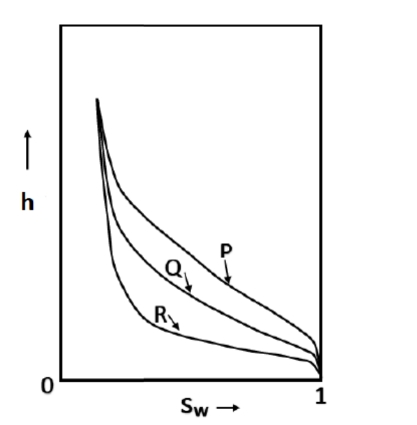
\includegraphics[width=0.2\linewidth]{figs/4.jpeg}
    \caption{}
    \label{fig:placeholder}
\end{figure}


  
\begin{enumerate}
\item (A) P: low density oil - water, Q: gas - water, R: high density oil - water
\item (B) P: gas - water, Q: low density oil - water, R: high density oil - water
\item (C) P: high density oil - water, Q: low density oil - water, R: gas - water
\item (D) P: gas - water, Q: high density oil - water, R: low density oil - water
\end{enumerate}


  \hfill{GATE PE 2020}
   
\item The fractional flow ($f_w$) versus water saturation ($S_w$) curve for an imbibition process (neglecting the capillary forces) in a given core for three different inclinations is shown in the figure.

\begin{figure}[h]
    \centering
    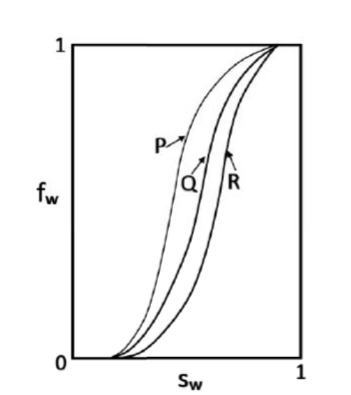
\includegraphics[width=0.3\linewidth]{figs/5.jpeg}
    \caption{}
    \label{fig:placeholder}
\end{figure}
Which one of the following is the correct representation of the fractional flow curves?

  
\begin{multicols}{2}
\begin{enumerate}
\item (A) P: Down-dip, Q: No-dip, R: Up-dip
\item (B) P: Down-dip, Q: Up-dip, R: No-dip
\item (C) P: No-dip, Q: Down-dip, R: Up-dip
\item (D) P: Up-dip, Q: No-dip, R: Down-dip
\end{enumerate}
\end{multicols}


  \hfill{GATE PE 2020}
   
\item Match the following:

\begin{table}[h!]
\centering
\[
\begin{array}{ll}
P.\; \text{Dynamic positioning} & I.\; \text{System for automatic position control} \\
Q.\; \text{Mooring}             & II.\; \text{Station keeping system} \\
R.\; \text{Jack-up}             & III.\; \text{Self-contained drilling rig on a floating barge} \\
S.\; \text{Semi-submersible platform} & IV.\; \text{Weight and buoyancy balance} \\
\end{array}
\]
\caption{Matching offshore drilling systems with their descriptions}
\label{tab:offshore}
\end{table}


  
\begin{multicols}{2}
\begin{enumerate}
\item (A) P-IV, Q-II, R-I, S-III
\item (B) P-III, Q-I, R-IV, S-II
\item (C) P-II, Q-IV, R-I, S-III
\item (D) P-II, Q-IV, R-III, S-I
\end{enumerate}
\end{multicols}


  \hfill{GATE PE 2020}
   
\end{enumerate}


\section*{GATE 2019 Petroleum Engineering}



\begin{enumerate}
\setcounter{enumi}{30} % Start from question 31

\item Match the following:

  \hfill{GATE PE 2020}
   
\item An exploratory well encountered three reservoir formations S1 (perfectly cemented), S2 (poorly cemented) and S3 (fractured). The Formation Factor ($F$) is governed by the equation $F = \alpha \phi^{-m}$, where '$\phi$' is the porosity and '$m$' is the cementation factor. The constant '$\alpha$', linked to tortuosity is assumed to be 1 for all formations. The log-log plot between Formation Factor ($F$) and porosity ($\phi$) is shown.
\begin{figure}[h]
    \centering
    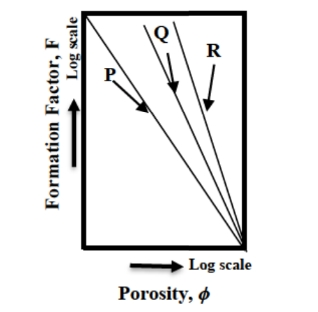
\includegraphics[width=0.2\linewidth]{figs/6.jpeg}
    \caption{}
    \label{fig:placeholder}
\end{figure}



Which one of the following represents the correct match of the formations with their respective plots?

  
\begin{multicols}{2}
\begin{enumerate}
\item (A) S1-P, S2-Q, S3-R
\item (B) S1-R, S2-P, S3-Q
\item (C) S1-P, S2-R, S3-Q
\item (D) S1-R, S2-Q, S3-P
\end{enumerate}
\end{multicols}


  \hfill{GATE PE 2020}
   
\item Typical parameters obtained in the pyrolysis experiment of the source rock materials are shown in the Figure. Which one of the following is NOT true about pyrolysis in source rock analysis?

\begin{figure}[h]
    \centering
    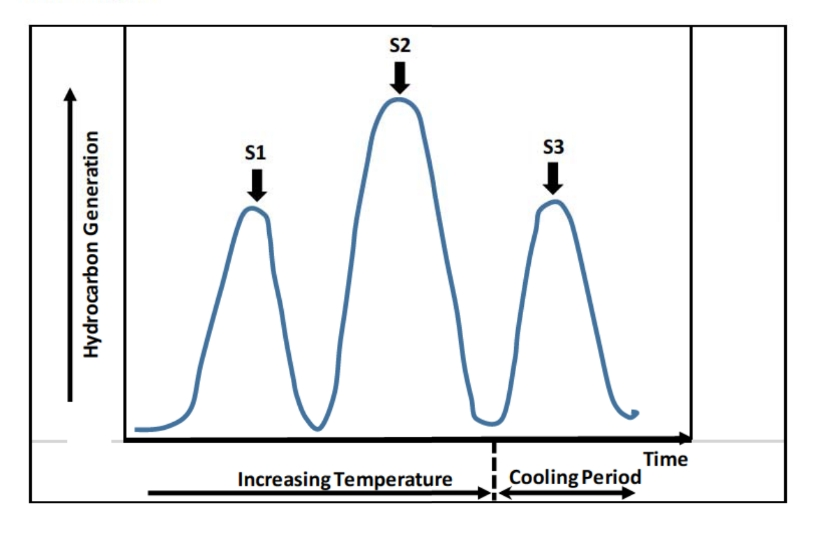
\includegraphics[width=0.4\linewidth]{figs/7.jpeg}
    \caption{}
    \label{fig:placeholder}
\end{figure}


  
\begin{enumerate}
\item (A) Peak S1 represents volatilization of existing hydrocarbons
\item (B) Peak S2 represents breakdown of kerogen and generation of hydrocarbons
\item (C) Peak S3 represents $T_{\text{max}}$, the temperature at which most hydrocarbons are generated
\item (D) S1/(S1+S2) represents the production index
\end{enumerate}

  \hfill{GATE PE 2020}
   
\item A single well encounters multiple clean sands of exactly the same thickness, porosity and permeability. $R_w$ is the formation fluid resistivity and $R_{\text{mf}}$ is the mud filtrate resistivity.

\begin{align}
\begin{array}{ll}
P.\; R_{\text{mf}} > R_w & I.\; \text{No deflection} \\
Q.\; R_{\text{mf}} = R_w & II.\; \text{Positive deflection} \\
R.\; R_{\text{mf}} < R_w & III.\; \text{Negative deflection} \\
\end{array}
\end{align}


Which one of the following matches the relation between $R_w$ and $R_{\text{mf}}$ to that of Self Potential (SP) log deflection?

  
\begin{multicols}{2}
\begin{enumerate}
\item (A) P-I, Q-III, R-II
\item (B) P-III, Q-I, R-II
\item (C) P-II, Q-I, R-III
\item (D) P-I, Q-II, R-III
\end{enumerate}
\end{multicols}


  \hfill{GATE PE 2020}
   
\item Which one of the following options is NOT a part of the mudlogs prepared by the drill-site geologist?

  
\begin{enumerate}
\item (A) Rate of Penetration (ROP)
\item (B) Chromatograph showing presence of C$_1$ to C$_5$ concentration
\item (C) Lithology from drill cutting and its interpretation
\item (D) Reservoir unit delineation based on volume of shale ($V_{sh}$)
\end{enumerate}


  \hfill{GATE PE 2020}
   
\item[Q.36] Match the following:

\begin{table}[h!]
\centering
\begin{align}
\begin{array}{ll}
P.\; \text{Location of storing the kelly on the trip} & I.\; \text{Mousehole} \\
Q.\; \text{Location of storing the next drill pipe} & II.\; \text{Rathole} \\
R.\; \text{Location of storing pump pressure gauges} & III.\; \text{Top drive} \\
S.\; \text{Rotational system that controls a drill string without a kelly} & IV.\; \text{Standpipe} \\
\end{array}
\end{align}
\caption{Drilling equipment and their locations/functions}
\end{table}


  
\begin{multicols}{2}
\begin{enumerate}
\item (A) P-II, Q-I, R-IV, S-III
\item (B) P-IV, Q-II, R-III, S-I
\item (C) P-II, Q-I, R-III, S-IV
\item (D) P-IV, Q-III, R-II, S-I
\end{enumerate}
\end{multicols}

  \hfill{GATE PE 2020}
   
\item A box contains 2 red and 3 black balls. Three balls are randomly chosen from the box and are placed in a bag. Then the probability that there are 1 red and 2 black balls in the bag, is .

   

  \hfill{GATE PE 2020}
   
\item The values of a function $f(x)$ over the interval [0,4] are given in the table below:

\begin{table}[h!]
\centering
\begin{align}
\begin{array}{|c|c|c|c|c|c|}
\hline
x & 0 & 1 & 2 & 3 & 4 \\
\hline
f(x) & 1 & 0.5 & 0.2 & 0.1 & 0.06 \\
\hline
\end{array}
\end{align}
\caption{Values of $f(x)$ for given $x$}
\end{table}

Then, according to the trapezoidal rule, the value of the integral $\int_{0}^{4} f(x) dx$ is  (round off to 2 decimal places).

   

  \hfill{GATE PE 2020}
   
\item Oil is produced at a constant rate from a well in a bounded reservoir. The variation of the bottom-hole pressure with time is shown in the given Table. The magnitude of the slope of the pressure vs time curve that you would use to find the drainage area is  psi/day (round off to 1 decimal place).

\begin{table}[h!]
\centering
\begin{align*}
\begin{array}{|c|c|c|c|}
\hline
\text{Time (days)} & \text{Pressure (psi)} & \text{Time (days)} & \text{Pressure (psi)} \\
\hline
0 & 3500 & 6 & 2512 \\
1 & 2864 & 7 & 2482 \\
2 & 2725 & 8 & 2452 \\
3 & 2644 & 9 & 2422 \\
4 & 2587 & 10 & 2392 \\
5 & 2542 & 11 & 2362 \\
\hline
\end{array}
\end{align*}
\caption{Pressure decline data over time}
\end{table}


  

  \hfill{GATE PE 2020}
   
\item In a core flood experiment of immiscible and incompressible displacement of oil ($\mu_0 = 1$ cP) with water ($\mu_w = 1$ cP), only axial flow is observed. The relative permeability of water is given by $k_{rw} = S_w^2$, where $S_w$ is water saturation. The relative permeability of oil is given by $k_{ro} = (1 - S_w)^2$. The gravity and capillary pressure are neglected. From the fractional flow and water saturation relationship, the saturation of water at the flood front is \_\_\_\_\_\% (round off to 1 decimal place).

   

  \hfill{GATE PE 2020}
   


\section*{GATE 2019 Petroleum Engineering}




\item In an oil well, the pressure at the gas oil contact (GOC) at a depth of 2000 m is 205 bar (gauge),as shown in the figure.
\begin{figure}[h]
    \centering
    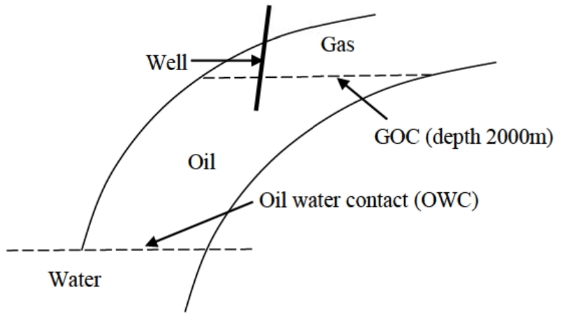
\includegraphics[width=0.5\linewidth]{figs/8.jpeg}
    \caption{}
    \label{fig:placeholder}
\end{figure}


The static oil pressure gradient is 0.08 bar/m in the pay zone. If a constant hydrostatic pressure gradient of 0.1 bar/m prevails throughout the subsurface, then the thickness of the oil column is:


  \hfill{GATE PE 2020}
 
\item Oil is produced at a constant rate of $10 \ \text{m}^3/\text{day}$ from a reservoir for $500$ days.  
The producing gas oil ratio (GOR) is constant at $10 \ \text{m}^3_{\text{gas}}/\text{m}^3_{\text{oil}}$ for the first $100$ days.  
Then, the producing gas oil ratio increases linearly and on the $500^{\text{th}}$ day the measured GOR is $50 \ \text{m}^3_{\text{gas}}/\text{m}^3_{\text{oil}}$.  
The cumulative produced gas oil ratio after $500$ days of production is \\\\ $\text{m}^3_{\text{gas}}/\text{m}^3_{\text{oil}}$ (round off to 1 decimal place).  
Assume that all volumes are measured at STP.  

  \hfill{GATE PE 2020}

 
\item A pressure build-up test was conducted in a well after $1000$ days of producing oil at a constant rate of $0.01 \ \text{reservoir-m}^3/\text{s}$.  
The two shut-in bottom-hole pressure readings taken at $0.5$ day and $1$ day after shut-in are $150 \times 10^5 \ \text{Pa}$ and $151 \times 10^5 \ \text{Pa}$, respectively.  
These pressure points correspond to the linear region of the Horner's plot.  
The reservoir thickness is $100 \ \text{m}$ and oil viscosity is $0.001 \ \text{Pa.s}$.  
The permeability of the reservoir is \\\\ mD (round off to 1 decimal place).  
[$1 \ \text{mD} = 10^{-15} \ \text{m}^2$]  


  \hfill{GATE PE 2020}

 
\item In an oil reservoir, the residual oil saturation in the volume flooded with polymer solution is $20\%$.  
The initial water saturation is $20\%$.  
The volumetric sweep efficiency is $50\%$.  
The maximum possible recovery factor for the reservoir is \_\_\_\ \% (round off to 1 decimal place).  

  \hfill{GATE PE 2020}
 
\item An electrical submersible pump (ESP) delivers well fluid with $100\%$ watercut.  
In the ESP, the impeller diameter is $0.1 \ \text{m}$ and speed is $3600 \ \text{rpm}$.  
The total head developed by the ESP is $300 \ \text{m}$ (water column height).  
If the stage efficiency of the ESP is $60\%$, then the minimum number of stages required is \\\\ (round off to nearest integer).  
[$g = 9.81 \ \text{m/s}^2$]  

  \hfill{GATE PE 2020}
 
\item In a counter flow heat exchanger, hot fluid enters at $100^\circ \text{C}$ and leaves at $50^\circ \text{C}$.  
Cold fluid enters at $30^\circ \text{C}$ and leaves at $40^\circ \text{C}$.  
If heat losses are ignored, then the logarithmic mean temperature difference (LMTD) is  $^\circ \text{C}$ (round off to 1 decimal place).  

  \hfill{GATE PE 2020}

 
\item A model porous block of cross-sectional area ($A$) and length ($L$) is made up of $N$ independent capillaries of equal radii ($r$) and length ($L$).  
The porosity of the block is $10\%$, and the permeability for a laminar, incompressible and steady state flow is $0.02 \ \text{mD}$.  
If the flow is only through the capillaries, then the value of $r$ is \_\_\_\ $\times 10^{-6} \ \text{cm}$ (round off to 1 decimal place).  
[$1 \ \text{mD} = 10^{-15} \ \text{m}^2$]  

  \hfill{GATE PE 2020}
 
\item A model porous medium of 5 cylindrical capillaries of radii varying from $60$ to $100 \ \mu\text{m}$ is subjected to Mercury Injection Capillary Pressure (MICP) treatment.  
The capillaries are being filled in an increasing order of their entry pressure.  
The magnitude of $(\sigma \cos \theta)_{\text{air-Hg}}$ is $367 \ \text{dyne/cm}$, where $\sigma$ is the interfacial tension and $\theta$ is the contact angle.  
The minimum applied mercury pressure to achieve $50\%$ mercury saturation in the sample is \_\_\_\ $\times 10^3 \ \text{dyne/cm}^2$ (round off to 1 decimal place).  

\begin{figure}[h]
    \centering
    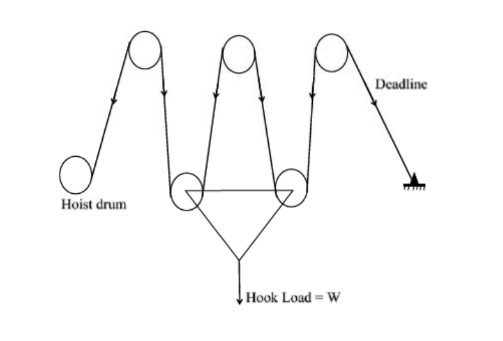
\includegraphics[width=0.5\linewidth]{figs/10.jpeg}
    \caption{}
    \label{fig:placeholder}
\end{figure}


  \hfill{GATE PE 2020}
   

\item The sonic log parameters from an exploratory well in a reservoir are as follows:  

Measured P-wave transit time ($\Delta t_{\text{log}}$) = $85  \mu\text{s/ft}$  
True resistivity ($R_{t}$) = $10 \ \Omega\text{-m}$  
Matrix transit time ($\Delta t_{\text{mat}}$) = $45 \ \mu\text{s/ft}$  
Fluid transit time ($\Delta t_{fl}$) = $205 \ \mu\text{s/ft}$  
Formation water resistivity at reservoir temperature ($R_{w}$) = $0.1 \ \Omega\text{-m}$  

The hydrocarbon saturation (in percentage) in the reservoir is \\\\ (round off to 1 decimal place).  

[Hint: Wyllie time average equation is $\Delta t_{\text{log}} = (1 - \phi)\Delta t_{\text{mat}} + \phi \Delta t_{fl}$ and formation water resistivity has the correlation $R_{w} = \frac{a}{\phi^{m}} R_{t} S_{w}^{n}$, where $S_{w}$ is water saturation, $\phi$ is porosity and $a = 1$]  

  \hfill{GATE PE 2020}
 
\item A vertical well of $8000 \ \text{ft}$ is producing below bubble point pressure. Oil and water each is produced at the rate of $500 \ \text{bbl/day}$. The indicated bottom hole pressure is $3000 \ \text{psia}$. If the same gas to liquid ratio (GLR) is maintained, using the given figure, the new bottom hole pressure at $5000 \ \text{ft}$ is \_\_\_\ psi.  
\begin{figure}[h]
    \centering
    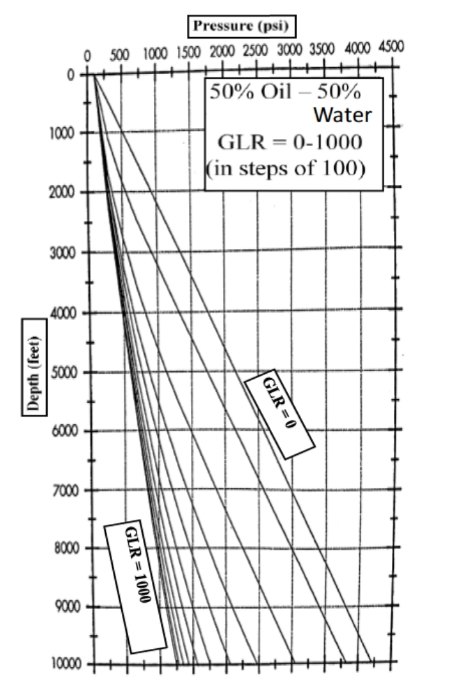
\includegraphics[width=0.3\linewidth]{figs/9.jpeg}
    \caption{}
    \label{fig:placeholder}
\end{figure}


  \hfill{GATE PE 2020}
 \newpage
\item In a drilling rig, the crown block and the traveling block have three and two sheaves, respectively. A single wireline connects the hoisting drum to the deadline anchor as shown in the figure. Neglect the weight of the pulleys and the wireline, and friction between the sheaves and wireline. The ratio of the deadline load to static crown load is  (round off to 2 decimal places).
\begin{figure}[h]
    \centering
    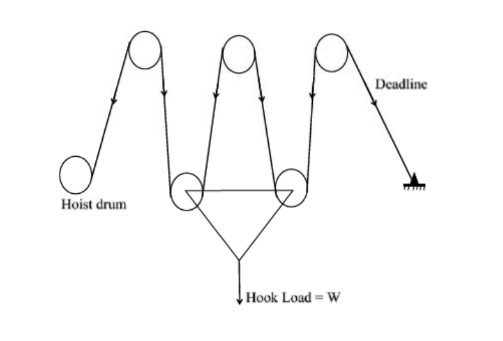
\includegraphics[width=0.3\linewidth]{figs/10.jpeg}
    \caption{}
    \label{fig:placeholder}
\end{figure}


  \hfill{GATE PE 2020}
 
\item Cement weighing $100  \text{kg}$ is mixed with $50 \ \text{liters}$ of water. The specific gravity of cement is $3.14$ and the density of water is $1000 \text{kg/m}^3$. Neglecting volume changes, the resulting density of the slurry is \\\\ $\text{kg/m}^3$ (round off to 1 decimal place).  

  \hfill{GATE PE 2020}
 
\item In an active water drive during a certain period, the rate of production and reservoir pressure remain constant. The water influx into the reservoir from the aquifer is $6000 \ \text{bbl/day}$. The surface oil and water production rates are $3000 \ \text{STB/day}$ and $1500 \ \text{STB/day}$, respectively. The current production gas to oil ratio is $825 \ \text{SCF/STB}$, and the formation volume factors at the current pressure for oil, water, and gas are $1.375 \ \text{bbl/STB}$, $1.04 \ \text{bbl/STB}$, and $0.007 \ \text{bbl/STB}$, respectively. The solution gas to oil ratio at the current pressure is \\\\ $\text{SCF/STB}$ (round off to 1 decimal place).  

  \hfill{GATE PE 2020}
 
\item In a water flooding experiment, the pressure gradients in the displacing and displaced phases are $400 \ \text{psi/ft}$ and $350 \ \text{psi/ft}$, respectively. Assume that the displacement front is stable in the absence of capillary and gravity forces. Consider that only water flows upstream and only oil flows downstream of the displacement front. Then, the mobility ratio for this immiscible displacement process is \\\\ (round off to 2 decimal places).  

  \hfill{GATE PE 2020}
 
\item In a pressure draw-down testing, the well bore flowing pressure ($P_{wf}$) is given by  

\begin{align}
P_{wf} = P_{i} - \frac{162.6 \, q \, \mu \, B}{k \, h} \left[ \log \left( \frac{k \, t}{\phi \, \mu \, c_{t} \, r_{w}^{2}} \right) - 3.23 + 0.87 \, S \right]
\end{align}

The following data is given in the oil field units:  

Initial reservoir pressure ($P_{i}$) = $5000 \ \text{psia}$  
Pressure after 1 hr of production ($P_{1hr}$) = $4000 \ \text{psia}$  
Oil flow rate ($q$) = $500 \ \text{STB/day}$  
Porosity ($\phi$) = $0.25$  
Viscosity of oil ($\mu$) = $2 \ \text{cP}$  
Formation volume factor of oil ($B$) = $1.2 \ \text{bbl/STB}$  
Formation thickness ($h$) = $20 \ \text{ft}$  
Total compressibility ($c_{t}$) = $30 \times 10^{-6} \ \text{psi}^{-1}$  
Well bore radius ($r_{w}$) = $0.3 \ \text{ft}$  

The slope of $P_{wf}$ versus $\log t$ is $-100 \ \text{psi/cycle}$. Then, the skin factor ($S$) for this well is \\\\ (round off to 1 decimal place).  

  \hfill{GATE PE 2020}
\end{enumerate}
 
\begin{center}
\textbf{\large --- END OF THE QUESTION PAPER ---}
\end{center}
\end{document}